%% LyX 2.3.2-2 created this file.  For more info, see http://www.lyx.org/.
%% Do not edit unless you really know what you are doing.
\documentclass[english]{upeeei}
\usepackage[utf8]{inputenc}
\usepackage{geometry}
\setcounter{secnumdepth}{3}
\setcounter{tocdepth}{3}
\usepackage[active]{srcltx}
\usepackage{float}
\usepackage{units}
\usepackage{graphicx}

\usepackage{units}
\usepackage[indent=1.5em]{parskip}
\usepackage{graphicx}
\usepackage{url}  
%\usepackage{stfloats}  
\usepackage{amsmath}   
\usepackage{array}
\usepackage{caption}
\usepackage{afterpage}
\usepackage{textcomp}
\usepackage{lscape}
\usepackage{stfloats}
\usepackage{hyphenat}
\usepackage{makeidx}
\usepackage{amssymb}
%\usepackage{underscore}
\fnbelowfloat
\usepackage{times}
\usepackage{multirow}
%\usepackage{float}
\usepackage{circuitikz}
\usepackage[backend=bibtex,bibstyle=ieee,citestyle=numeric-comp]{biblatex}
\addbibresource{bibfile.bib}
\usepackage{pgfplots}
%\usepackage{arydshln}
\pgfplotsset{width=7cm,compat=1.5.1}
\renewcommand*{\bibfont}{\small}

\newcolumntype{L}[1]{>{\raggedright\let\newline\\\arraybackslash\hspace{0pt}}m{#1}}
\newcolumntype{C}[1]{>{\centering\let\newline\\\arraybackslash\hspace{0pt}}m{#1}}
\newcolumntype{R}[1]{>{\raggedleft\let\newline\\\arraybackslash\hspace{0pt}}m{#1}}

\newcommand\ddfrac[2]{\frac{\displaystyle #1}{\displaystyle #2}}
\pgfplotsset{compat=1.14}

\makeatletter

%%%%%%%%%%%%%%%%%%%%%%%%%%%%%% LyX specific LaTeX commands.
\providecommand{\LyX}{L\kern-.1667em\lower.25em\hbox{Y}\kern-.125emX\@}
%% Because html converters don't know tabularnewline
\providecommand{\tabularnewline}{\\}

\@ifundefined{showcaptionsetup}{}{%
 \PassOptionsToPackage{caption=false}{subfig}}
\usepackage{subfig}
\makeatother

\usepackage{babel}
\usepackage[hidelinks]{hyperref}
\begin{document}
%%% UP EEEI undergraduate project template
%% v0.1 by Louis P. Alarcon 11/22/2011
%%
%% LyX template - use with the following files:
%% 	uct10_new.clo, uct11_new.clo, uct12_new.clo, upeeei.cls, upeeei.layout
%%

%% Place project title here
\title{Comparing NCHW and NHWC Mappings in FPGA-Based CNN Inference Accelerators Using Weight-Stationary Systolic Arrays} 

%%
%% Author information


\author{
Gavin Christian Montevirgen\\ 2023-04094\\ \emph{BS Computer Engineering} \and
Jonelle Cyrille Bino\\ insert here\\ \emph{BS Computer Engineering} \and
Collette Mala\~{n}gen\\ 2023-03303\\ \emph{BS Computer Engineering}
}


%%
%% Month and year of submission/graduation
\degreeyear{2026} 
\degreesemester{December} 

% Put your advisers here:
\chair{Anastacia Alvarez\\
Adelson Chua
}
\othermembers{
Carl Aries Oliva\\\
Jose Francois Abedejos\\
Allen Jason Tan
}
\numberofmembers{6}


\field{Computer Engineering} 
\campus{Diliman} 

\maketitle

% uncomment the following four lines once you need to submit your approved 198/199 manuscript after the final assessment
%\newgeometry{verbose,tmargin=0.5in,bmargin=1in,lmargin=0.5in,rmargin=0.5in}
%\newpage
\thispagestyle{empty}

\noindent \begin{center}
\begin{tabular}{c}

\includegraphics[width=0.625in]{EEE Documentation/198_199_frontmatter/UP_logo_maroon.jpg}\tabularnewline
UNIVERSITY OF THE PHILIPPINES\tabularnewline
\end{tabular}
\par\end{center}

\vspace*{\fill}

% replace [Course] with specific course
\begin{center}
Bachelor of Science in [Course] Engineering
\par\end{center}

\vspace*{\fill}

% student names
\begin{center}
[Student/s Name]\\\par
[Student/s Name]\\\par
%[Student/s Name]\\\par
\end{center}

% project title
\begin{center}
[Project Title]
\par\end{center}

\vspace*{\fill}

\begin{center}
Undergraduate Project Adviser:\\\par
\par\end{center}

% adviser/s
\begin{center}
[Adviser/s Name]\\\par
[Adviser/s Name]\\\par
%[Adviser/s Name]\\\par
\end{center}

\begin{center}
Electrical and Electronics Engineering Institute \\\par
University of the Philippines Diliman
\par\end{center}

\vspace*{\fill}

\begin{center}
Undergraduate Project Reader:\\\par
\par\end{center}

\begin{center}
[Examiner/s Name] 
\par\end{center}

\begin{center}
Electrical and Electronics Engineering Institute \\\par
University of the Philippines Diliman 
\par\end{center}

\vspace*{\fill}

\begin{center}
Date of Submission 
\par\end{center}

\begin{center}
[Date of Final Manuscript submission]
\par\end{center}

\vspace*{\fill}

\begin{center}
Permission is given for the following people to have access to this thesis: 
\\\par\end{center}

\noindent \begin{center}
\begin{tabular}{|l|c|}
\cline{1-1} 
Circle one or more concerns: \hspace*{1cm}I\qquad{}P\qquad{} C & \multicolumn{1}{c}{}\tabularnewline
\hline 
Available to the general public & Yes/No\tabularnewline
\hline 
Available only after consultation with author/thesis adviser & Yes/No\tabularnewline
\hline 
Available only to those bound by confidentiality agreement & Yes/No\tabularnewline
\hline 
\multicolumn{1}{l}{\hspace*{10cm}} & \multicolumn{1}{c}{\hspace*{2cm}}\tabularnewline
\end{tabular}
\par\end{center}

Students\textquoteright{} signature/s: \\

Signature/s of undergraduate project advisers:
%% Note: You may decrease the amount of vertical spacing indicated in \vspace*{} in the case that you need to include more than three advisers.
\chapter*{Approval Sheet}
\thispagestyle{empty}
% Replace [Project Title] and [Student Name/s] with project title and student name/s respectively
In partial fulfillment of the requirements for the degree of [Course], this project
entitled ``[Project Title]'', prepared and submitted by [Student Name/s], is hereby recommended for approval.

\vspace*{1cm}

% replace [Adviser Name] with adviser name
\begin{tabular}{llc}
 &  & \tabularnewline
\cline{1-1} \cline{3-3} 
[Adviser Name 1] &  & Date\tabularnewline
Adviser &  & \tabularnewline
 &  & \tabularnewline
 
% uncomment the following lines for a second adviser
% &  & \tabularnewline
%\cline{1-1} \cline{3-3} 
%[Adviser Name 2] &  & Date\tabularnewline
%Adviser &  & \tabularnewline
% &  & \tabularnewline
 
% uncomment the following lines for a third adviser
% &  & \tabularnewline
%\cline{1-1} \cline{3-3} 
%[Adviser Name 3] &  & Date\tabularnewline
%Adviser &  & \tabularnewline
% &  & \tabularnewline
 
\hspace*{10cm} & \hspace*{1cm} & \hspace*{2cm}\tabularnewline
\end{tabular}

\vspace*{1cm}

% replace [Course] with course name
\noindent Accepted in partial fulfillment of the requirements for
the degree of [Course].

\vspace*{1cm}
% replace [Panel Member/s Name] and [Institute Director Name] with examiner name and the name of the institute director respectively
\begin{tabular}{llc}
 &  & \tabularnewline
\cline{1-1} \cline{3-3} 
[Panel Member/s Name] &  & Date\tabularnewline
Panel Member &  & \tabularnewline
 &  & \tabularnewline
\hspace*{10cm} & \hspace*{1cm} & \hspace*{2cm}\tabularnewline
 &  & \tabularnewline
\cline{1-1} \cline{3-3} 
[Institute Director Name] &  & Date\tabularnewline
Director, Electrical and Electronics Engineering Institute &  & \tabularnewline
\end{tabular}

%\newpage
\chapter*{University Permission Page}
\thispagestyle{empty}


I hereby grant the University of the Philippines non-exclusive worldwide,
royalty-free license to reproduce, publish, and public distribute
copies of this work in any form subject to the provisions of applicable
laws, the provisions of the UP IPR policy and any contractual obligations,
as well as more specific permission marking on the Title Page.\\

\noindent Specifically I grant the following rights to the University:
\begin{itemize}
\item to upload a copy of the work in the theses database of the college/school/institute/department
and in any other databases available on the public internet; 
\item to publish the work in the college/school/institute/department journal,
both in print and electronic or digital format and online; and 
\item to give open access to above-mentioned work, thus allowing \textquotedblleft fair-use\textquotedblright{}
of the work in accordance with the provisions of the Intellectual
Property Code of the Philippines (Republic Act No. 8293), especially
for teaching, scholarly, and research purposes. 
\end{itemize}
\vspace*{2cm}

\begin{tabular}{llc}
 &  & \tabularnewline
\cline{1-1} \cline{3-3} 
[Student Name/s and Signature] &  & Date\tabularnewline
 &  & \tabularnewline
 &  & \tabularnewline
 
% &  & \tabularnewline
%\cline{1-1} \cline{3-3} 
%[Student Name/s and Signature] &  & Date\tabularnewline
% &  & \tabularnewline
% &  & \tabularnewline

% &  & \tabularnewline
%\cline{1-1} \cline{3-3} 
%[Student Name/s and Signature] &  & Date\tabularnewline
% &  & \tabularnewline
% &  & \tabularnewline

 \hspace*{10cm} & \hspace*{1cm} & \hspace*{2cm}
\end{tabular}

%\newpage
\chapter*{Acknowledgment}
\thispagestyle{empty}

Insert acknowledgement message here\\

[Name]

[Student Number]

[Course]

%\restoregeometry

\begin{abstract} 

%Your abstract goes here...
Convolutional neural networks (CNNs) are widely used for vision and spatial tasks in machine learning and are typically accelerated with systolic array architectures. Feeding 4-dimensional matrix data to the systolic arrays requires reshaping into a 1-dimensional memory space, implying different mapping schemes. NCHW unrolls the input-spatial dimensions (height and width) first while NHWC unrolls the input-channel (C) dimension first. Previous hardware accelerator studies have examined data layout trade-offs, but comparisons of NCHW- and NHWC-based mappings in FPGA-based systolic arrays remain limited. This study compares NCHW- and NHWC-based implementations for CNN inference, using weight-stationary systolic arrays targeting the Artix-7 XC7A200T FPGA on the Nexys Video board. The comparison explores how these architectures affect execution time, resource utilization, power, energy, latency, and estimated maximum operating frequency. The study aims to optimize the layer dimensions and hardware configurations under which each implementation is efficient and explain the architectural mechanisms responsible for their performance and hardware-cost trade-offs.

\abstractsignature\end{abstract}

\begin{frontmatter} 
\setlength{\parskip}{0pt}
\tableofcontents{}
\listoffigures
\listoftables
\end{frontmatter} 

\def\MASTERDOC{true}
\cleardoublepage{}
\chapter{Introduction\label{cha:Introduction}}

\section{Background of Neural Networks}
\label{section:sec01_01}
Artificial Intelligence (AI) has become a foundational technology across modern computing, allowing systems to perform cognitive tasks ranging from perception to decision-making. Machine Learning (ML) has emerged as a core branch of AI specializing in learning statistical patterns to make predictions directly from data without explicit programmed instructions. As datasets and problem complexity have become increasingly complicated, deep learning, a subset of ML, has become the staple to learn complex patterns directly from large amounts of data as it can automatically extract features from raw inputs like images, audio, and text. 

An Artificial Neural Network (ANN) is a computational model used for deep learning systems consisting of interconnected artificial neurons that imitate the neurons in human brains and forms layers to learn with pattern recognition from training data. Among different neural network architectures, Convolutional Neural Networks (CNNs) have emerged as the standard for vision and spatial tasks due to their high feature-extraction capability. However, CNN inference and training requires rigorous multiply-accumulate (MAC) operations that overwhelm standard general-purpose Central Processing Units (CPUs). In order to handle the computational load and accelerate deep learning tasks, specialized machine learning accelerators have been developed. Although these accelerators can reach high peak compute density, they lose efficiency because of memory bottlenecks since energy consumption and execution latency are dominated by off-chip and on-chip memory accesses rather than arithmetic computations. Consequently, studies regarding architectural optimizations focus on exploiting data reuse to minimize data movement.

\section{Field-Programmable Gate Array Implementations}
\label{section:sec01_02}

When developing specialized ML accelerators, Field-Programmable Gate Arrays (FPGAs) help provide a reconfigurable hardware platform well-suited for implementing under strict area, power, and memory constraints. Unlike general-purpose CPUs and Graphics Processing Units (GPUs) which rely on fixed memory hierarchies and large off-chip capacities to support large models, FPGAs allow direct customization of both hardware logic and on-chip memory. This flexibility makes FPGAs more suitable for exploring much denser and resource-efficient accelerator designs.

\section{Systolic Arrays and Image-to-Column}
\label{section:sec01_03}
Systolic array architectures accelerate deep learning workloads by interconnecting MAC units into a 2D grid, allowing input data and partial sums to pulse from one processing element (PE) to another, minimizing expensive memory accesses. To map multi-dimensional CNN convolutions efficiently onto systolic arrays, the Image-to-Column (im2col) method can be used. Flattening and unrolling 4D Input Feature Maps (IFMaps) and weight filters into 2D matrices help transform sliding-window convolution operations into standard General Matrix Multiplication (GEMM) operations. By converting convolutions into GEMM, the data can be streamed rhythmically across the systolic array's 2D grid of PEs, maximizing PE utilization, simplifying control logic, and enabling high spatial and temporal data reuse across rows and columns.

\begin{figure} [H]
    \centering
    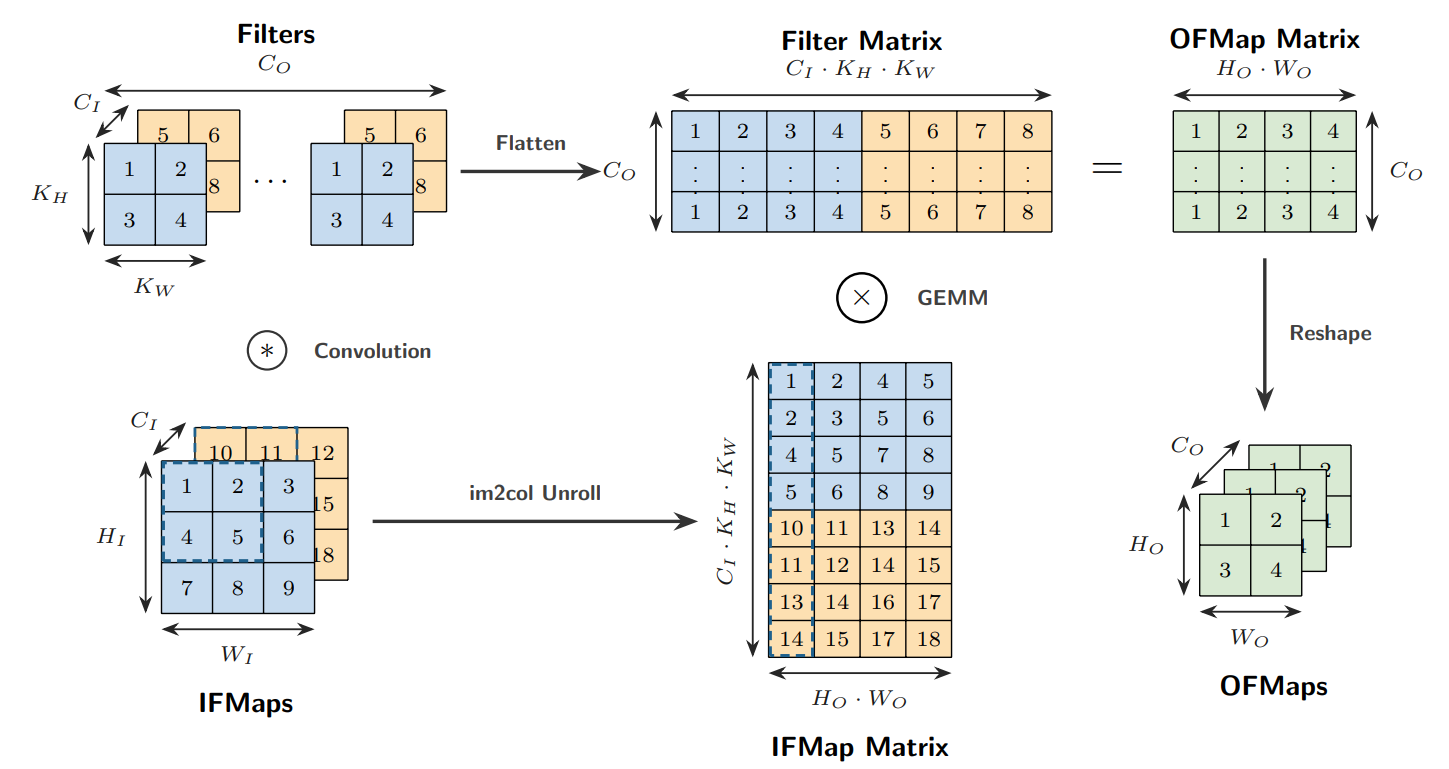
\includegraphics[scale=0.5]{figures/im2col.png}
    \caption{Transforming Convolution to GEMM using im2col}
    \label{fig:S11_graph}
\end{figure}

While standard or explicit im2col simplifies the convolutions into GEMM, it requires lowering the entire 4D IFMap in software before execution and overlapping receptive-field values to be duplicated into memory multiple times, increasing memory requirements. To mitigate off-chip memory expansion, on-the-fly im2col dynamically assembles lowered matrix tiles inside dedicated on-chip scratchpad buffers immediately before feeding the systolic array. However, it still incurs redundant on-chip memory storage, staging delays, and extra buffer-management logic. To overcome these limitations entirely, implicit im2col can be used which uses Address Generation Units (AGUs) to calculate the matrix coordinates from the original IFMap to stream activations directly into systolic arrays without materializing the matrix memory and avoiding data duplication.

\section{Research Gaps}
\label{section:sec01_04}
Since implicit im2col relies on real-time address calculation rather than physical data duplication, the underlying memory layout of the 4D tensor regulates memory accesses, bank conflicts, and AGU complexity.  Two of the most notable layouts are NHWC (Batch, Height, Width, Channel), which groups all channels of the same pixel together in memory, and NCHW (Batch, Channel, Height, Width), which groups pixels of the same channel together. While existing studies have examined the comparisons of NHWC and NCHW layouts across various CNN architectures, how they behave within FPGA-based weight-stationary systolic arrays utilizing implicit im2col remains largely uncharacterized. To bridge this gap, this study aims to conduct a systematic evaluation of NHWC- and NCHW-based implicit im2col architectures across varying layer dimensions, systolic array sizes, and on-chip memory capacities to analyze their trade-offs in execution performance, PE utilization, FPGA resource utilization, memory efficiency, and energy consumption.


\cleardoublepage{}

\chapter{Related Work\label{cha:RRW}}

This chapter details the different works \textbf{related} to your topic. The rule of thumb in writing this section is to start from a broad range of topics and narrowing it down to your topic of interest.

Note that this is a \emph{review} so you need to identify the \emph{problems} of the work you are reviewing. Critically criticize their work, identify what is common between them and differentiate your proposed solution from them. This is the most difficult part of your proposal.

\section{Different Mapping Implementations}
\label{section:sec02_01}

\section{NHWC and NCHW Comparisons in CPUs/GPUs}
\label{section:sec02_02}

\cleardoublepage{}




\chapter{Problem Statement and Objectives \label{cha:ProbStatement}}

\section{Problem Statement}

The problem is stated here in one coherent paragraph summarizing your RRW.

\section{Objectives of the Project}
\label{section:sec_obj}
The \textbf{concrete} goals of the project are stated here. Define the metrics that will measure the success of your project. It will be the basis for your examiner for your 198 grade.

\section{Scopes and Limitations}
\label{scopes}
This optional section defines the scope of the project. The project must be doable in 16 weeks and this section ensures that limit to be possible for you. The stated goals from section \ref{section:sec_obj} may not be achievable within 16 weeks if you don't define the scope.

\cleardoublepage{}



\chapter{Methodology\label{cha:Methodology}}

We will implement and test two architectures on the Nexys Video board~\cite{digilentNexysVideo}, which uses an
Artix-7 XC7A200T FPGA. One architecture uses NCHW implicit im2col lowering and the
other uses NHWC. We will run layer-dimension sweeps and hardware configuration sweeps on both
architectures. Two model benchmarks will also be run on an MNIST CNN and All-CNN-C on CIFAR-10. The
performance of each architecture will be measured in terms of latency, clock cycles, processing
element (PE) utilization, FPGA resource utilization, and board energy.

\section{Tensor dimension labeling conventions}

The dimensions of each tensor will be labeled as shown in Table~\ref{tab:tensor-dimensions}.

\begin{table}[H]
    \centering
    \begin{tabular}{|c|L{5.15in}|}
        \hline
        \textbf{Tensor} &
        \textbf{Dimensions} \\\hline
        Input &
        Batch size (N), input channels (C), input height (H), input width (W) \\\hline
        Kernel &
        Number of filters (K), channels per filter (C), kernel height (R), kernel width (S) \\\hline
        Output &
        Batch size (N), output channels (K), output height (P), output width (Q) \\\hline
    \end{tabular}
    \caption{Tensor dimension labeling conventions}
    \label{tab:tensor-dimensions}
\end{table}

\section{Implementations}

\subsection{Lowering methods}

Figures~\ref{fig:nchw-lowering} and~\ref{fig:nhwc-lowering} show the two implicit im2col lowering
methods as described by Zhou et al.~\cite{zhou2021implicit}.

\begin{samepage}
\subsubsection{NCHW}

Each row in the lowered input matrix is a convolution window for one output position. In each row,
the height and width dimensions are contiguous. Meanwhile, each column of the lowered kernel matrix
is a flattened filter with filter height and width contiguous.

\nopagebreak
\begin{figure} [H]
    \centering
    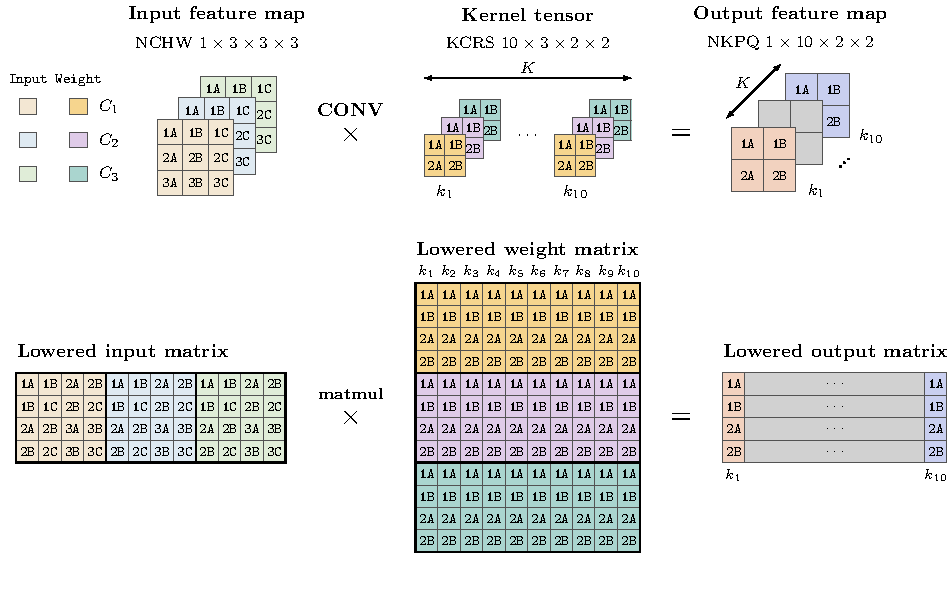
\includegraphics[width=\linewidth]{figures/methodology/nchw-lowering.pdf}
    \caption{NCHW lowering.}
    \label{fig:nchw-lowering}
\end{figure}
\end{samepage}

\begin{samepage}
\subsubsection{NHWC}

NHWC uses the same lowered matrix as NCHW with its columns reordered such that the input channels
are contiguous. The rows of the lowered kernel matrix are also rearranged accordingly.

\nopagebreak
\begin{figure} [H]
    \centering
    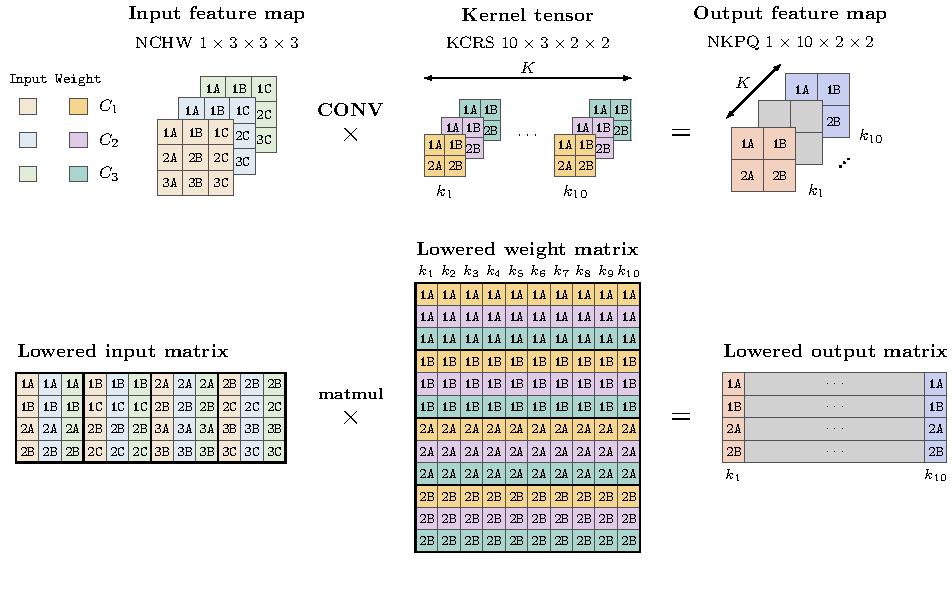
\includegraphics[width=\linewidth]{figures/methodology/nhwc-lowering.pdf}
    \caption{NHWC lowering.}
    \label{fig:nhwc-lowering}
\end{figure}
\end{samepage}

\subsection{Architectures}

\subsubsection{Common configurations}

Table~\ref{tab:common-configurations} lists the settings identical in each paired comparison
between the two architectures.

\begin{table}[H]
    \centering
    \ssp % Restore the class single spacing after array redefines tabular.
    \begin{tabular}{|L{1.45in}|L{4.55in}|}
        \hline
        \textbf{Parameter} &
        \textbf{Setting} \\\hline
        External memory tensor order &
        NCHW\footnotemark[\numexpr\value{footnote}+1\relax] inputs; KCRS weights; NKPQ outputs \\\hline
        Data types &
        Signed INT8 inputs and weights, signed INT32 accumulations \\\hline
        Dataflow &
        Weight-stationary \\\hline
        On-chip memory &
        Identical; 1:1:4 split between input, kernel, and output SRAMs \\\hline
        Systolic array size &
        Identical \\\hline
        Output-write path &
        INT32 accumulation \(\to\) add INT32 bias \(\to\) requantization (multiply, shift, round, INT8
            saturation) \(\to\) ReLU. Bias addition, requantization, and ReLU are applied when enabled. \\\hline
        Layer sequencing &
        Fetches layer descriptors\footnotemark[\numexpr\value{footnote}+2\relax] sequentially \\\hline
        Tiling method &
        Same tile traversal order \\\hline
    \end{tabular}
    \caption{Common configurations}
    \label{tab:common-configurations}
\end{table}
\stepcounter{footnote}
\footnotetext{%
  The difference in NCHW and NHWC is seen in the systolic array feeding and on-chip mapping
}
\stepcounter{footnote}
\footnotetext{%
  Layer descriptors are fetched from and stored in DDR memory. Layer descriptors contain the
  following information needed per layer: layer dimensions, stride, padding, dilation,
  input/weight/output base addresses, output-write settings, a last flag indicating the current
  layer is the last layer
}

\subsubsection{Tiling loop}

Both architectures use the same output tile traversal order.

\begin{quote}
% Use the template's compact single-spaced font for the tiling loop.
\AddToHookNext{env/verbatim/begin}{\let\ssp\scriptsizessp}
\begin{verbatim}
for each output image:
  for each output-channel block:
    for each output row:
      for each horizontal output tile:
        for each input-channel block:
          load the required input patch and corresponding weights
          convolve the input patch with the weights via the systolic array
          accumulate partial sums for the output tile
        apply enabled output-write settings
        store the output tile
\end{verbatim}
\end{quote}

The tile size limits are described in Table~\ref{tab:tile-size-limits}.

\begin{table}[H]
    \centering
    \begin{tabular}{|c|c|}
        \hline
        \textbf{Tile dimension} &
        \textbf{Limit} \\\hline
        Output-channel block &
        Number of PE columns \\\hline
        Output rows &
        One row per tile \\\hline
        Tile width &
        Input and output SRAM capacities \\\hline
        Input-channel block size &
        Input and weight SRAM capacities; number of PE rows \\\hline
    \end{tabular}
    \caption{Tile size limits}
    \label{tab:tile-size-limits}
\end{table}

\begin{samepage}
\subsubsection{NCHW}

Figure~\ref{fig:nchw-architecture} describes the NCHW accelerator’s architecture. DDR memory
will hold the layer descriptors and tensors, and the DMA engine will move data between DDR and the
accelerator. The topmost modules’ jobs are described in the figure. The \texttt{conv\_core} module
contains the systolic array, the banked SRAMs, the weight loader, the activation feeder, address
generator, and output accumulators. For each output position, the address generator computes the
bank and word address needed to fetch the input activation required per PE row. The activation
feeder contains the bank service logic to handle bank conflicts and the crossbar to route data from
the banks to the two activation vector slots. These slots are pipelined such that one is filled
while the other feeds the systolic array. These slots are to lessen stalls from bank conflicts and
retries.

\nopagebreak
\begin{figure} [H]
    \centering
    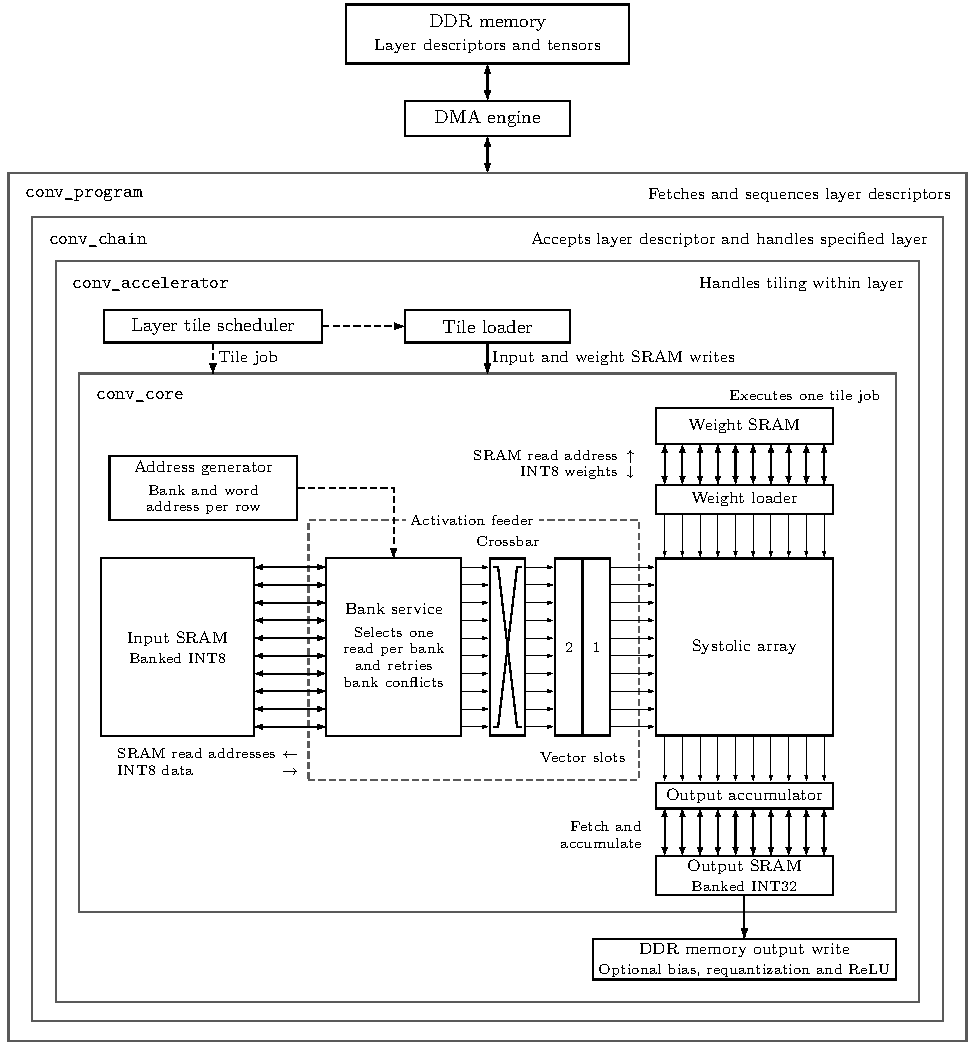
\includegraphics[width=.79\linewidth]{figures/methodology/nchw-architecture.pdf}
    \caption{NCHW accelerator.}
    \label{fig:nchw-architecture}
\end{figure}
\end{samepage}

\begin{samepage}
Figure~\ref{fig:nchw-array} shows how the NCHW accelerator would execute the convolution in
Figure~\ref{fig:nchw-lowering}. In the systolic array, the weights of the first pass are loaded. A
second pass is required to handle the last two rows of the lowered kernel matrix. An output channel
is dedicated to each PE column. In the input SRAM, we see the input activations needed for the first
and second rows of the lowered input matrix. These contribute to the output-channel block’s first
output row. They are also ordered in a way that reduces bank conflicts, a technique discussed in
Zhou et al.~\cite{zhou2021implicit}. Lastly, we see the vector slots: slot 1 has the input
activations for the output position 1A of the output row loaded while slot 2 has the input
activations for output position 1B.

\nopagebreak
\begin{figure} [H]
    \centering
    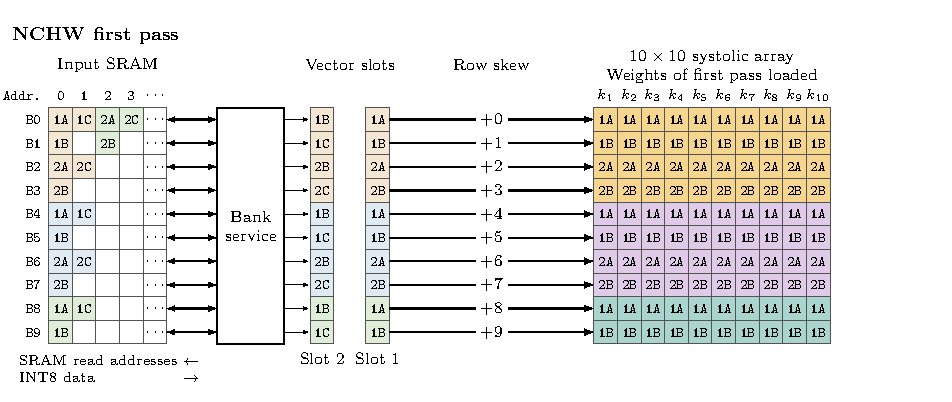
\includegraphics[width=\linewidth]{figures/methodology/nchw-array.pdf}
    \caption{NCHW SRAM and systolic array.}
    \label{fig:nchw-array}
\end{figure}
\end{samepage}

\begin{samepage}
\subsubsection{NHWC}

Figure~\ref{fig:nhwc-architecture} describes the NHWC accelerator’s architecture. The DDR
memory and DMA engine function the same way as described in NCHW. The module \texttt{conv\_core} has
the same main blocks, with differences in the activation feeder and the address generator. The
activation feeder is simpler, no longer needing the bank service logic, crossbar, and activation
vector slots due to how NHWC feeds the input feature map, dedicating one input channel per PE row.

\nopagebreak
\begin{figure} [H]
    \centering
    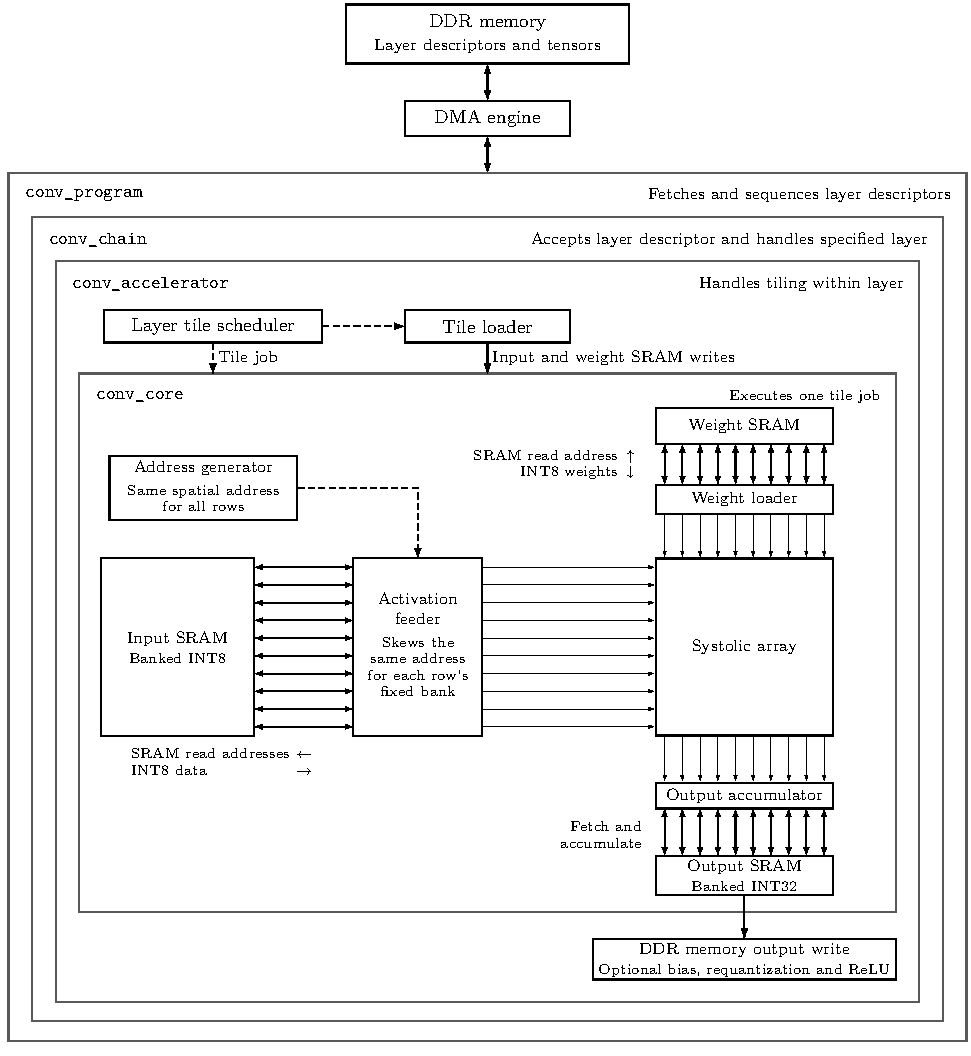
\includegraphics[width=.79\linewidth]{figures/methodology/nhwc-architecture.pdf}
    \caption{NHWC accelerator.}
    \label{fig:nhwc-architecture}
\end{figure}
\end{samepage}

\begin{samepage}
Figure~\ref{fig:nhwc-array} shows how the first tap of the convolution in
Figure~\ref{fig:nhwc-lowering} maps onto the systolic array and input SRAMs. In the systolic
array, the first tap’s weights are loaded. The next
tap would be the next kernel position across all filters, labeled 1B in the lowered kernel matrix.
Like in NCHW, an output channel is dedicated per PE column. Each input channel has its own PE row,
meaning input elements do not jump between PE rows, which is why there is no need for the crossbar,
bank service logic, and two activation vector slots.

\nopagebreak
\begin{figure} [H]
    \centering
    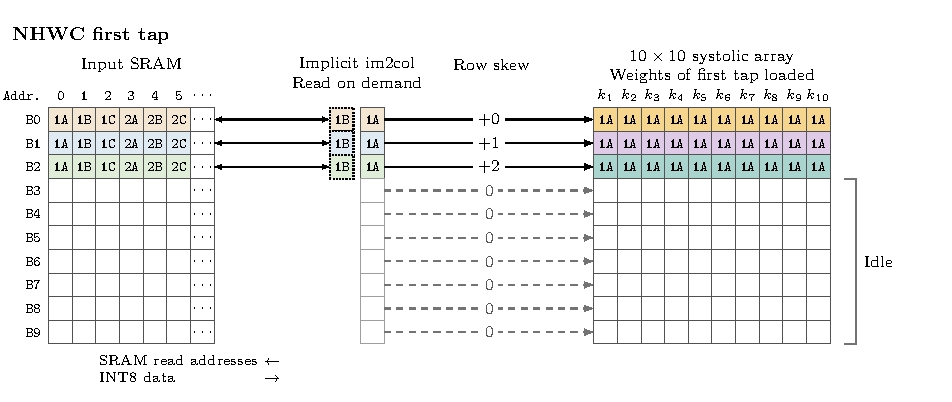
\includegraphics[width=\linewidth]{figures/methodology/nhwc-array.pdf}
    \caption{NHWC SRAM and systolic array.}
    \label{fig:nhwc-array}
\end{figure}
\end{samepage}

\section{Implementation on the Nexys Video Board}

\subsection{Board build and DDR}

Vivado 2026.1 will be used and the Nexys Video Artix-7 will be targeted. Its onboard DDR3 memory
will be used. The same DDR controller settings and memory layout will be used across paired
comparisons to ensure fairness. Fit, timing, and correctness failures will be recorded.

\subsection{Clocks to test}

The sweeps and model benchmarks will be run on both architectures at a common clock 20 MHz and each
architecture’s highest verified clock. The highest verified clock will be the highest tested clock
that meets routed timing and pass board correctness checks. The post-route WNS will be used to
estimate this. The Vivado documentation states the following formula for the max
frequency~\cite{amd2026frequency}:

\[
  \begin{aligned}
    F_{\mathrm{max}} &= \frac{1000}{T - \mathrm{WNS}} \\[.5em]
    T &= \text{target clock period in ns} \\
    \mathrm{WNS} &= \text{worst negative slack in ns}
  \end{aligned}
\]

\subsection{Test automation}

The host script will program the FPGA, queue the sweep and model runs, save timing results,
counters, and power traces. FPGA GPIO signals will be used to mark the start and end of each
measurement window.

\section{Sweeps}

Layer-dimension sweeps and hardware configuration sweeps will be done on both architectures. The
same randomly-generated tensors will be tested to ensure fairness in comparison. All cases have
padding at 0, dilation at 1, and stride at 1. The split of 1:1:4 between the input,
kernel, and output SRAMs in Table~\ref{tab:common-configurations} will also apply.

\subsection{Layer dimensions sweep}

For the sweeps in Table~\ref{tab:layer-sweeps}, the hardware configuration will be kept constant
at a 10~×~10 systolic array and 15 KiB of on-chip memory.

\begin{table}[H]
    \centering
    \begin{tabular}{|C{1.38in}|C{1.12in}|C{1.15in}|L{2.05in}|}
        \hline
        \textbf{Sweep} &
        \textbf{Input size} &
        \textbf{Kernel size} &
        \textbf{Input \(\to\) output channels} \\\hline
        input-channel sweep &
        32~×~32 &
        3~×~3 &
        input-channels: 1-32; \newline output channels: 3 and 10 \\\hline
        output-channel sweep &
        32~×~32 &
        3~×~3 &
        output-channels: 1-32; \newline input channels: 3 and 10 \\\hline
        spatial-size sweep &
        8~×~8, 16~×~16, 32~×~32 &
        3~×~3 &
        3 \(\to\) 3, 3 \(\to\) 10,\newline 10 \(\to\) 3, 10 \(\to\) 10 \\\hline
        kernel size sweep &
        32~×~32 &
        1~×~1, 3~×~3, 5~×~5, 7~×~7 &
        3 \(\to\) 3, 3 \(\to\) 10,\newline 10 \(\to\) 3, 10 \(\to\) 10 \\\hline
    \end{tabular}
    \caption{Layer dimensions sweep}
    \label{tab:layer-sweeps}
\end{table}

\subsection{Hardware configuration sweep}

All permutations in Table~\ref{tab:hardware-sweep} will be tested. The kernel size will be held constant at
3~×~3.

\begin{table}[H]
    \centering
    \begin{tabular}{|c|c|c|C{1.47in}|}
        \hline
        \textbf{Input size} &
        \textbf{Array sizes} &
        \textbf{On-chip memory} &
        \textbf{Input \(\to\) output channels} \\\hline
        8~×~8, 32~×~32 &
        8~×~8, 10~×~10, 16~×~16 &
        7.5, 15, 30 KiB &
        3 \(\to\) 16\newline 3 \(\to\) 64\newline 64 \(\to\) 16\newline 64 \(\to\) 64 \\\hline
    \end{tabular}
    \caption{Hardware configuration sweep}
    \label{tab:hardware-sweep}
\end{table}

\subsection{Supporting decisions for sweep choices}

\subsubsection{Input/output channels}

Since PE array utilization is sensitive to the number of input/output channels, it’s given the
finest sweep. This sweep shows us where each architecture leads in power, energy, latency, and cycle
count.

\subsubsection{Kernel size and spatial size}

These were varied at the chosen input and output channel counts to see how kernel and spatial size
affect performance at high/low input/output channel counts.

\subsubsection{Systolic array size and SRAM sweep}

Similar to how SCALE-Sim~\cite{samajdar2020scalesim} studied varying array size and SRAM capacity,
we vary these parameters to see how they may affect cycle count and DDR traffic on both
architectures given the same layer.

\subsection{Total cases}

Summing the cases from Tables~\ref{tab:layer-sweeps} and~\ref{tab:hardware-sweep} and counting
overlapping cases once, we get 215 runs per architecture, making 430 runs. Then, with two
clock conditions to test on, we get 860 board cases.

\section{Model benchmarks}

Benchmarks on two models, MNIST CNN and All-CNN-C on CIFAR-10, will be done to test how the two
architectures’ performance tradeoffs carry over to actual networks. Tests will be run on the same
hardware configuration of a 10~×~10 systolic array with 15 KiB on-chip memory. Training and
calibration of the networks will be done via Keras on Python.

\subsection{Network details}

\subsubsection{MNIST}

Table~\ref{tab:mnist-network} summarizes the network. This is based on a University of Florida
example~\cite{ufMnist}. The MNIST network classifies a 28~×~28 grayscale image of a white digit on a
black background.

\begin{table}[H]
    \centering
    \begin{tabular}{|C{.65in}|c|c|c|c|c|C{.67in}|}
        \hline
        \textbf{Layer} &
        \textbf{Input (NCHW)} &
        \textbf{Kernel (KCRS)} &
        \textbf{Output (NKPQ)} &
        \textbf{Stride} &
        \textbf{Pad} &
        \textbf{Nonlinear func} \\\hline
        Conv1 &
        1 × 1 × 28 × 28 &
        16 × 1 × 8 × 8 &
        1 × 16 × 11 × 11 &
        2 &
        0 &
        ReLU \\\hline
        Conv2 &
        1 × 16 × 11 × 11 &
        8 × 16 × 5 × 5 &
        1 × 8 × 4 × 4 &
        2 &
        0 &
        ReLU \\\hline
        Flatten\footnotemark[\numexpr\value{footnote}+1\relax] &
        1 × 8 × 4 × 4 &
        — &
        1 × 128 × 1 × 1 &
        — &
        — &
 \\\hline
        Dense32 &
        1 × 128 × 1 × 1 &
        32 × 128 × 1 × 1 &
        1 × 32 × 1 × 1 &
        1 &
        0 &
        ReLU \\\hline
        Dense10 &
        1 × 32 × 1 × 1 &
        10 × 32 × 1 × 1 &
        1 × 10 × 1 × 1 &
        1 &
        0 &
        Argmax \\\hline
    \end{tabular}
    \caption{MNIST CNN network}
    \label{tab:mnist-network}
\end{table}
\stepcounter{footnote}
\footnotetext{%
  Only explicitly defined during the Keras training process. In the accelerator, CONV2’s output
  will be treated as Dense32’s input directly
}

The dense or fully-connected layers were mapped to a convolution as described in Abdelfattah et
al~\cite{abdelfattah2018dla}. The flattened input is treated as the channels at one spatial
position, with each output neuron computed by a 1~×~1 filter that spans all input channels.

\subsubsection{All-CNN-C for CIFAR-10}

Table~\ref{tab:all-cnn-c-network} summarizes the network. This is based on Springenberg et al.’s section
on All-CNN-C~\cite{springenberg2015allcnn}. CIFAR-10 maps a 32~×~32 RGB image into ten classes: airplane,
automobile, bird, cat, deer, dog, frog, horse, ship, truck~\cite{krizhevskyCifar}.

\begin{table}[H]
    \centering
    \begin{tabular}{|C{.65in}|c|c|c|c|c|C{.67in}|}
        \hline
        \textbf{Layer} &
        \textbf{Input (NCHW)} &
        \textbf{Kernel (KCRS)} &
        \textbf{Output (NKPQ)} &
        \textbf{Stride} &
        \textbf{Pad} &
        \textbf{Nonlinear func} \\\hline
        Conv1 &
        1 × 3 × 32 × 32 &
        96 × 3 × 3 × 3 &
        1 × 96 × 32 × 32 &
        1 &
        1 &
        ReLU \\\hline
        Conv2 &
        1 × 96 × 32 × 32 &
        96 × 96 × 3 × 3 &
        1 × 96 × 32 × 32 &
        1 &
        1 &
        ReLU \\\hline
        Conv3 &
        1 × 96 × 32 × 32 &
        96 × 96 × 3 × 3 &
        1 × 96 × 16 × 16 &
        2 &
        1 &
        ReLU \\\hline
        Conv4 &
        1 × 96 × 16 × 16 &
        192 × 96 × 3 × 3 &
        1 × 192 × 16 × 16 &
        1 &
        1 &
        ReLU \\\hline
        Conv5 &
        1 × 192 × 16 × 16 &
        192 × 192 × 3 × 3 &
        1 × 192 × 16 × 16 &
        1 &
        1 &
        ReLU \\\hline
        Conv6 &
        1 × 192 × 16 × 16 &
        192 × 192 × 3 × 3 &
        1 × 192 × 8 × 8 &
        2 &
        1 &
        ReLU \\\hline
        Conv7 &
        1 × 192 × 8 × 8 &
        192 × 192 × 3 × 3 &
        1 × 192 × 6 × 6 &
        1 &
        0 &
        ReLU \\\hline
        Conv8 &
        1 × 192 × 6 × 6 &
        192 × 192 × 1 × 1 &
        1 × 192 × 6 × 6 &
        1 &
        0 &
        ReLU \\\hline
        Conv9 &
        1 × 192 × 6 × 6 &
        10 × 192 × 1 × 1 &
        1 × 10 × 6 × 6 &
        1 &
        0 &
        ReLU \\\hline
        Global average pooling &
        1 × 10 × 6 × 6 &
        — &
        1 × 10 × 1 × 1 &
        – &
        – &
        Argmax \\\hline
    \end{tabular}
    \caption{All-CNN-C network}
    \label{tab:all-cnn-c-network}
\end{table}

The global average pooling layer in the end will be mapped to a convolution by treating
Conv9’s 1~×~10~×~6~×~6 output as a 10~×~1~×~6~×~6 input, then convolving it with a
1~×~1~×~6~×~6 filter filled with ones at stride 1, dilation 1, and zero padding. The output will
then be 10~×~1~×~1~×~1, with one INT32 sum per class. We take the argmax of these sums. This method
adapts Abdelfattah et al.’s approach~\cite{abdelfattah2018dla}.

\subsection{Training}

Table~\ref{tab:training-settings} summarizes the training details for both models to be tested.

\begin{table}[H]
    \centering
    \begin{tabular}{|L{1.25in}|L{1.82in}|L{2.85in}|}
        \hline
        \textbf{Training setting} &
        \textbf{MNIST CNN} &
        \textbf{All-CNN-C on CIFAR-10} \\\hline
        Dataset source &
        Keras~\cite{kerasMnist} &
        Keras~\cite{kerasCifar10} \\\hline
        Dataset allocation\newline (training / validation / test) &
        48,000 / 12,000 / 10,000\newline 0.2 validation
            split~\cite{khan2024mnist,ridgeway2019recombination,luza2022radiation} &
        45,000 / 5,000 / 10,000\newline 500 images per class held out for validation (Bingham and
            Miikkulainen, 2022, Appendix A.5)~\cite{bingham2022parametric} \\\hline
        Preprocessing &
        Scale pixel values to [0, 1] &
        Global contrast normalization then ZCA whitening fitted on the training images (Goodfellow et
            al., §5.2)~\cite{goodfellow2013maxout} \\\hline
        Data augmentation &
        None &
        Random horizontal flips and random translations of up to five pixels along each axis
            (Springenberg et al., §3.2.1)~\cite{springenberg2015allcnn} \\\hline
        Regularization &
        None &
        L2 regularization of 0.001 to weights\newline 0.2 dropout probability on input, then 0.5 after
            Conv 3 and Conv 6 (Springenberg et al., §3.2.1)~\cite{springenberg2015allcnn} \\\hline
        Optimizer &
        Adam &
        Stochastic gradient descent, momentum 0.9 (Springenberg et al.,
            §3.2.1)~\cite{springenberg2015allcnn} \\\hline
        Batch size &
        128 &
        128 (Bingham and Miikkulainen, 2023, Table 5)~\cite{bingham2023surrogate} \\\hline
        Learning rate and epochs &
        40 epochs with Adam learning rate at 0.001 (Keras Adam default)~\cite{kerasAdam} &
        Test initial learning rates 0.01, 0.05, 0.1, 0.25. Multiply by 0.1 after epochs 200, 250,
            300.\newline 350 epochs total per learning rate (Springenberg et al.,
            §3.2.1)~\cite{springenberg2015allcnn} \\\hline
        Checkpoint selection &
        Pick lowest validation loss (epoch 17) &
        Pick learning rate and checkpoint with lowest validation loss \\\hline
    \end{tabular}
    \caption{Training settings}
    \label{tab:training-settings}
\end{table}

Upon completion of training, each convolutional and dense layer will have learned weights and one
bias per output channel..

\subsection{Calibration, quantization, and exporting}

The trained networks, which use floating-point data, will require calibration and quantization
before they can be run in the two architectures.

For calibration, we run each trained floating-point model through inference on its training images
to obtain the largest absolute values for the input and each intermediate output we quantize. We
find the largest absolute weight in each layer directly from the trained weights. We divide these
largest absolute values by 127 to get the input, weight, and output scales. When a layer’s output is
used as the input to the next layer, a scaling factor is computed for that layer using the equation
below. The factor converts the accumulated result to the next layer’s input
scale~\cite{jacob2018quantization}:

\[\text{scaling factor} = \frac{\text{input scale} \times \text{weight scale}}{\text{output scale}}\]

On export, we convert the trained weights to INT8 by dividing them by their weight scale and
rounding. We also convert each bias to INT32 by dividing it by the bias scale (input scale x weight
scale) and rounding. The computed scaling factors per layer will be approximated using an integer
multiplier and a right shift as well, as shown below~\cite{jacob2018quantization}:

\[\text{scaling factor} = 2^{-(\text{right shift})} \times \text{multiplier}\]

Both architectures will use the same exported weights, biases, and scales for each model.

\subsection{Input image preparation}

For each model, one test image will be selected, preprocessed, and saved for testing. For MNIST, the
pixel values of the 28~×~28 grayscale image will be scaled to [0,1]. For All-CNN-C, we apply global
contrast normalization to its 32~×~32 RGB image, followed by a ZCA whitening transform fitted on the
training images. Each preprocessed image will then be quantized to INT8 by dividing its values by
the model’s input scale, rounding, and clipping to the quantized range. The same saved inputs will
be used for both architectures and clock conditions.

\section{Metrics and paired analysis}

We will measure the accuracy of the models, and the correctness, latency, PE utilization, cycle
counts, and FPGA resource utilization of our architectures.

\subsection{Correctness}

The outputs of the sweeps and model benchmarks will be tested to match against independent integer
references.

\subsection{Model accuracy}

We will report the accuracy of each model against each one’s full test set for both its
floating-point and its quantized models.

\subsection{Latency measurements}

FPGA GPIO signals will be used to mark the start and end of the measurement windows mentioned.

\subsubsection{Layer-dimension and hardware configuration sweeps}

The measurement for each layer case will be from the layer descriptor acceptance to assertion of the
accelerator’s layer done signal. For each case, architecture, and clock condition, we will run 50
warm-ups followed by 2,500 timed runs~\cite{ji2026c2fdeploy}.

\subsubsection{Model benchmarks}

The measurement will be from the first layer descriptor acceptance to the accelerator’s class-valid
signal. The class-valid signal means argmax at the last layer has chosen a winning class. For each
model, architecture, and clock condition, we will run 5 warm-ups followed by 50 timed runs on the
same test image~\cite{ji2026c2fdeploy}.

\subsubsection{Statistics to report}

We will report mean, standard deviation, and median across timed runs~\cite{ji2026c2fdeploy}

\subsection{PE utilization in core execution}

PE utilization will be measured during core execution. The below formula describes PE utilization:

\[\text{PE utilization} = \frac{\text{useful MACs}}{\text{physical PEs} \times \text{total core execution cycles}}\]

A multiply-and-accumulate (MAC) operation is considered useful if its input is within bounds (not a
padding zero) and contributes to the output. We will report total useful MACs, useful MACs per
full-layer cycle, and useful MACs per byte transferred in DDR.

\subsection{Cycle counts and memory traffic}

For each layer, hardware counters will record cycle counts and the cycles spent in the following
phases: planning, input loads, weight loads, bias loads, core execution cycles, output writes, and
tile transitions. Inputs and weights are loaded from DDR memory to the SRAMs, while outputs are
written from the output SRAM back to DDR memory. We will also include DDR wait cycles in phases
where they occur and record them separately. We will track NCHW bank conflicts and retries
separately. We will check that the phase counts sum to the total cycle count.

We will also count the output tiles and bytes read from and written to DDR. For the accelerator’s
input, weight, and output SRAM, we will measure reads, writes, and peak occupied bytes for each.

\subsection{FPGA Resource Utilization}

For each hardware configuration tested on the board, we will report the FPGA’s LUT, flip-flop, BRAM,
and DSP usage.

\subsection{Energy measurement}

Board energy will be measured with the same measurement windows used in latency. Voltage across the
Nexys Video’s 12V input and current into the board will be measured simultaneously. Their product
will be integrated over the measurement window to get energy. We will also get mean active board
power by dividing the energy by the length of the GPIO-marked window.

\subsection{Paired analysis}

For every case, we will show the raw values, which mapping leads or ties in each metric, and the
percentage change relative to NCHW. We will compare cycle counts and latency at the common 20MHz
clock and at each build’s highest verified clock. We will favor lower cycles, latency, traffic,
resource use, measured energy, and higher PE utilization. We will use the cycle phases, output tile
counts, and stalls to explain the differences between NCHW and NHWC.

\cleardoublepage{}




\chapter{Preliminary Findings\label{cha:Prelims}}

This is an \emph{optional} chapter that reports on the feasibility of your project. You may be required by your adviser to have a preliminary work ready by the end of the semester.

\cleardoublepage{}




\chapter{Project Schedule and Deliverables\label{cha:Project-Sked}}


\section{Gantt Chart }

A Gantt Chart detailing the different steps to complete your project. Try to cram as much detail into this chart as possible and also show a clear division of tasks if you will work on a project as a group.

\section{Halfway-point Deliverables}

Define the expected output upon halfway of the semester, i.e., at the end of 8 weeks. This will aid your examiner and adviser on determining if you should still continue your 198 or fail you pre-emptively.

\cleardoublepage{}

\printbibliography


\end{document}
